In questo capitolo si mostra la classificazione mediante \textit{SVM} con kernel trick.\\
Anceh in questo caso si utilizzano le tecniche di PCA per la dimensionality reduction, come nel caso della regressione logistica.\\
I kernel utilizzati sono quello lineare, gaussiano e la funzione sigmoide.\\
Il modello SVM è incluso nella classe \textit{SVC} di scikit-learn.\\
Un problema notato nei capitoli precedenti è che le due classi non sono molto divisibili da un decision boundary lineare. Infatti ci si aspettano prestazioni migliori utilizzando il kernel gaussiano o con la funzione sigmoide.
\begin{lstlisting}
from sklearn.svm import SVC

pca = PCA(n_components=2)

principal_components = pca.fit_transform(X)
principalDF = pd.DataFrame(data=principal_components,
columns=['principal component 1', 'principal component 2'])

finalDf = pd.concat([principalDF, brain_tumor_data[['Target']]], axis=1)

X = finalDf.drop("Target", axis=1)
Y = finalDf["Target"].values

X_train, X_test, Y_train, Y_test = train_test_split(X, Y, test_size=0.3)

svc = SVC(kernel="linear", probability=True)
svc.fit(X_train, Y_train)
score_linear2d = svc.score(X_test, Y_test)
print("=========== PCA 2D ===========")
print("ACCURACY WITH LINEAR KERNEL: " + str(score_linear2d))

svc = SVC(kernel="rbf", probability=True)
svc.fit(X_train, Y_train)
score_rbf2d = svc.score(X_test, Y_test)
print("ACCURACY WITH GAUSSIAN KERNEL: " + str(score_rbf2d))

svc = SVC(kernel="sigmoid", probability=True)
svc.fit(X_train, Y_train)
score_sigmoid2d = svc.score(X_test, Y_test)
print("ACCURACY WITH SIGMOID KERNEL: " + str(score_sigmoid2d))
\end{lstlisting}
Nella classe SVC vengono settati i campi \textit{kernel} e \textit{probability}. Il campo kernel permette di specificare quale tipo di kernel utilizzare per misurare la somiglianza tra due sample. Il campo probability viene settato a \textit{true} per includere il calcolo della probabilità di accuratezza delle predizioni. Ciò rallenta di non poco l'algoritmo ma può essere utile per avere un ulteriore feedback sulle prestazioni del modello.\\
\section{Conclusioni su classificazione con SVM}
\begin{figure}[h]
	\centering   	
	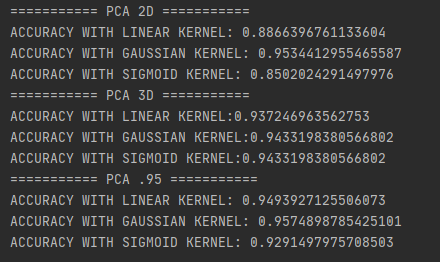
\includegraphics[width=100mm]{image/svmresults.png}
	\caption{Risultati stampati sulla console Python}
\end{figure}
Come ci si aspettava la tecnica migliore risulta quella ottenuta con kernel gaussiano e con PCA 95\%.\\
Come si può notare però, il contributo maggiore viene fornito dal tipo di kernel. Infatti per il dataset in questione il kernel più performante è quello gaussiano a prescindere dal tipo di PCA utilizzato. Infatti nei tre casi di PCA si nota che le prestazioni del modello SVM con kernel gaussiano cambiano di poco, mentre il tipo di tecnica PCA utilizzata può influire molto se si utilizzano kernel lineari o sigmoidali.